%!TEX root = GRoutes.tex
%%%%%%%%%%%%%%%%%%%%%%%%%%%%%%%%%%%%%%%%%%%%%%%%%%%%%%%%%%%%%%%%%%%%%%%
\chapter{Gráfok}\label{ch:ALAP}
%%%%%%%%%%%%%%%%%%%%%%%%%%%%%%%%%%%%%%%%%%%%%%%%%%%%%%%%%%%%%%%%%%%%%%%

\begin{osszefoglal}
	Ebben a fejezetben a későbbiekben használt fogalmakat fogom definiálni.
	
\end{osszefoglal}

%%%%%%%%%%%%%%%%%%%%%%%%%%%%%%%%%%%%%%%%%%%%%%%%%%%%%%%%%%%%%%%%%%%%%%%
\section{Alapfogalmak}\label{sec:ALAP:adatelem}

Egy gráf \(G = (V(G),E(G)\) vagy \(G = (V,E))\) két véges halmazból áll. \(V(G)\) vagy \(V\), egy nem üres halmaz, melynek az elemeit csúcsoknak nevezzük, ezek alkotják a gráf csúcsait. \(E(G)\) vagy \(E\), egy halmaz, melynek elemeit éleknek nevezzük, ezek alkotják a gráf éleit, úgy, hogy minden \(e \in E\) élet meghatároz egy rendezetlen csúcs-pár \((u,v)\), melyeket \(e\) csúcsainak nevezünk \cite{gt_alg_india}.

\begin{description}
	\setlength{\itemsep}{0.04mm}
	\item[rend] -- definíció szerint a \(G\) gráf rendje \(|V| = n\)
	\item[méret] -- definíció szerint a \(G\) gráf mérete \(|E| = m\)
	\item[hurokél] -- olyan él, melynek mindkét végpontja megegyezik
	\item[többszörös él] -- ha két csúcsot több él köt össze, akkor ezeket többszörös, vagy párhuzamos éleknek nevezzük
	\item[egyszerű gráf] -- azon gráf, amely nem tartalmaz sem hurokélt, sem többszörös éleket
	\item[teljes gráf] -- egy egyszerű gráf, amelynek minden különböző csúcs-párját összeköti egy él. Egy teljes gráf \(n(n-1)/2\) éllel rendelkezik. Ha a teljes gráf csúcsai \(v_1, v_2, \ldots, v_n\), akkor az élek halmaza megadható a következőképpen:
	\begin{equation}
	E = \{(v_i,v_j): v_i \neq v_j;\;\;\;i,j = 1,2,3\dots, n\}
	\end{equation}
	\item[irányított gráf] -- olyan gráf, ahol az éleket rendezett \((u,v)\) csúcspárok határozzák meg (számít, hogy melyik a kezdő- és végpont)
	\item[részgráf] -- Legyen \(H\) egy gráf, csúcsainak halmaza \(V(H)\), éleinek halmaza \(E(H)\), hasonlóan \(G\) egy gráf, csúcsainak halmaza \(V(G)\) és éleinek halmaza \(E(G)\). \(H\) részgráfja \(G\)-nek, ha \(V(H) \subseteq V(G)\) és \(E(H) \subseteq E(G)\).
	\item[séta] -- a csúcsok és élek váltakozó véges sorozata, mely csúccsal kezdődik és csúccsal végződik, valamint minden csúcsot egy vele szomszédos él követ és fordítva
	\item[vonal] -- az a séta, melyben az élek nem ismétlődnek.
	\item[út] -- az a séta, melyben a csúcspontok nem ismétlődnek.
	\item[kör] -- egy nem-triviális%
	\footnote{ %
		hossza nagyobb, mint 0
	}  %
 zárt vonal, amelynek a kezdő- és belső pontjai nem ismétlődnek.
	\item[Hamilton-út] -- egy \(G\) gráf azon útja, mely minden csúcsot magába foglal
\end{description}

%%%%%%%%%%%%%%%%%%%%%%%%%%%%%%%%%%%%%%%%%%%%%%%%%%%%%%%%%%%%%%%%%%%%%%%
\section{Részgráf izomorfizmus probléma}\label{sec:ALAP:adatelem}

A részgráf izomorfizmus egy komputacionális probléma, adottak a \(H\) és \(G\) gráfok, és el kell dönteni, hogy létezik-e \(G\)-nek olyan részgráfja, amely izomorf \(H\)-val. Ennek bizonyítása egy NP-teljes feladat \cite{gt_problem}.

%%%%%%%%%%%%%%%%%%%%%%%%%%%%%%%%%%%%%%%%%%%%%%%%%%%%%%%%%%%%%%%%%%%%%%%
\section{Gráfok színezése}\label{sec:ALAP:adatelem}

Egy gráf színezése azt jelenti, hogy a csúcsaihoz (vagy az éleihez) színeket rendelünk (legtöbbször egy számmal reprezentáljuk), úgy, hogy két bármely két szomszédos csúcs (vagy él) különböző színű legyen.

%%%%%%%%%%%%%%%%%%%%%%%%%%%%%%%%%%%%%%%%%%%%%%%%%%%%%%%%%%%%%%%%%%%%%%%
\section{Útproblémák}\label{sec:ALAP:adatelem}

\subsection{Hamilton-kör probléma}

A Hamilton-kör egy gráfban egy olyan kör, mely áthalad a gráf összes csúcsán. Mivel egy kör, minden csúcson egyszer fog áthaladni, kivéve az elsőt, ami egyben az utolsó is. Egy gráfot Hamilton-gráfnak nevezünk, ha tartalmaz Hamilton-kört.

Ore tétele apalján egy egyszerű gráf \(G = (X,E)\), \(n \leq 3\) csúccsal Hamilton gráf, ha \(d(x) + d(y)  \geq n\), minden nem szomszédos \(x,y \in X\) csúcsra.

Ebből kifolyólag egy gráfban a Hamilton-kör létezése elméleti szemszögből nem egy egyszerú probléma, de gyakorlati szemszögből sem, mivel NP%
\footnote{ %
	nem determinisztikusan polinomiális
}  %
-teljes. Az utazó ügynök problémája magába foglalja a Hamilton-kör létezését a gráfban.

\subsection{Minimális feszítőfa}

Egy \(fa\) egy olyan gráf, amely összefüggő és nem tartalmaz köröket. Bármely összefüggő \(G\) gráfban a feszítőfa \(G\)-nek egy olyan részgráfja, amely fa, és tartalmazza \(G\) összes csúcsát. A minimális feszítőfát meghatározhatjuk Prim algoritmusa vagy Kruskal algoritmusa segítségével.

Prim algoritmusa: kezdjük bármelyik csúccsal, majd válasszuk ki a hozzá tartozó legkisebb súllyal rendelkező élet. Minden iterációban kiválasztjuk az eddig vizsgált csúcsokhoz tartozó élek közül a legkisebb súllyal rendelkező élet, majd hozzáadjuk az eddig kapott fához az eddig nem vizsgált csúcspontjával együtt. Ezt addig folyatjuk, míg az összes csúcsot megvizsgáltuk.

\subsection{Kínai postás-probléma}

Egy \(G\) gráfban találjuk meg a legrövidebb zárt sétát, amely minden élen legalább egyszer halad át. Egy optimális megoldást találni úgy irányított, mint irányítatlan gráfban, ez a probléma is NP-teljes.

\subsection{Königsbergi hidak problémája}

Königsberg városában volt hét híd (\ref{fig:ALAP:sm1} ábra), amely összekötött két szigetet a város két partjával és egymással. A lakosok megpróbáltak úgy sétálni, hogy minden hídon egyszer és csakis egyszer haladjanak át, és érjenek vissza a kezdőpontba. Ez soha senkinek nem sikerült: Euler magyarázta meg egy 1736-ban írt cikkben, hogy ez miért nem lehetséges.

Egy Euler-út egy gráfban egy olyan út, amely minden élet magába foglal, egyszer és csakis egyszer. Egy Euler-út zárt, ha ugyanabban a csúcsban végződik, mint ahonnan elindul, egyébként nyíltnak nevezzük.

Egy gráf akkor és csakis akkor tartalmaz zárt Euler-utat, ha minden csúcshoz páros számú él tartozik, valamint minden él ugyanahhoz a komponenshez tartozik. Egy gráf akkor és csakis akkor tartalmaz nyílt Euler-utat, ha pontosan két csúcshoz tartozik páratlan számú él, és minden él egyazon komponenshez tartozik.

\begin{figure}
	\centering
	\setlength{\abovecaptionskip}{0pt}
	\setlength{\belowcaptionskip}{0pt}
	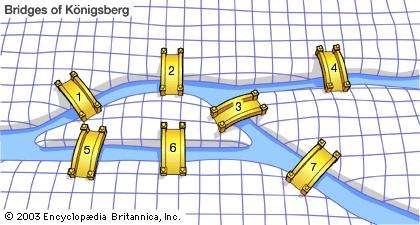
\includegraphics[width=0.9\textwidth, scale=0.9]{images/konigsberg}
	\caption[]%
	{Königsbergi hidak\\
		{\white .}\hfill{forrás: }\url{https://cdn.britannica.com/s:700x450/77/74877-004-6D15B0BD.jpg/}}
	\label{fig:ALAP:sm1}
\end{figure}

\subsection{Legrövidebb út probléma}

Legrövidebb út problémájára egy megoldás Dijkstra algoritmusa, mely visszatéríti a legrövidebb utat a kiinduló csúcsból az összes többi csúcsba. Negatív súlyú élek esetén nem működik. Az algoritmus komplexitása \(O(n^2)\), ahol \(n\) a csúcsok száma.

